\newcommand{\picscale}{0.5}
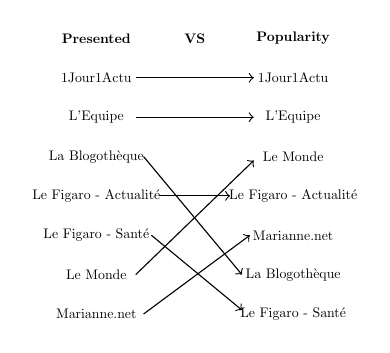
\begin{tikzpicture}[scale=\picscale, every node/.style={scale=\picscale}]
    % Columns.
    \node at (0  , 0) {\bf Presented};
    \node at (2.5, 0) {\bf VS};
    \node at (5  , 0) {\bf Popularity};
    
    % As presented.
    \node at (0,-1) {1Jour1Actu};
    \node at (0,-2) {L'Equipe};
    \node at (0,-3) {La Blogoth\`{e}que};
    \node at (0,-4) {Le Figaro - Actualit\'{e}};
    \node at (0,-5) {Le Figaro - Sant\'{e}};
    \node at (0,-6) {Le Monde};
    \node at (0,-7) {Marianne.net};
    
    % As popular.
    \node at (5,-1) {1Jour1Actu};
    \node at (5,-2) {L'Equipe};
    \node at (5,-3) {Le Monde};
    \node at (5,-4) {Le Figaro - Actualit\'{e}};
    \node at (5,-5) {Marianne.net};
    \node at (5,-6) {La Blogoth\`{e}que};
    \node at (5,-7) {Le Figaro - Sant\'{e}};
    
    % Arrows between presented and popular.
    \draw [->] (1,-1)   --   (4,-1);
    \draw [->] (1,-2)   --   (4,-2);
    \draw [->] (1.2,-3) --   (3.7,-6);
    \draw [->] (1.6,-4) --   (3.4,-4);
    \draw [->] (1.4,-5) --   (3.7,-6.9);
    \draw [->] (1,-6)   --   (4,-3.1);
    \draw [->] (1.2,-7) --   (3.9,-5);
    
\end{tikzpicture} 